\documentclass[a4paper, 12pt]{book}

\usepackage{graphicx}
\usepackage{wrapfig}
\usepackage[font=small,labelfont=bf]{caption}
\usepackage{index}
\usepackage{hyperref}
\usepackage{amsmath}
\usepackage{xcolor}
\usepackage{listings}
\usepackage{xepersian}

\captionsetup[figure]{font=small}

\makeatletter
\renewcommand\@endpart{\vfil
              \if@twoside
                \null
                \thispagestyle{empty}%
                \newpage
              \fi
              \if@tempswa
                \twocolumn
              \fi}
\makeatother

\renewcommand{\baselinestretch}{1.6}

\newcommand{\lrbold}[1]{\lr{\textbf{#1}}}
\newcommand{\lrboldit}[1]{\lr{\textbf{\textit{#1}}}}
\newcommand{\lrit}[1]{\lr{\textit{#1}}}


\settextfont{B Yekan}
\setlatintextfont[Scale=1.2]{Arial}
\DefaultMathsDigits

% -- define code style

\definecolor{customblue}{RGB}{246, 247, 246}
\definecolor{keywordcolor}{RGB}{157, 0, 236}
\definecolor{codepurple}{rgb}{0.58,0,0.82}
\definecolor{stringcolor}{RGB}{0, 130, 0}
\definecolor{light-gray}{gray}{0.95}
\lstdefinestyle{C++Style}{%
  backgroundcolor=\color{customblue},
  breaklines=true,
  basicstyle=\footnotesize\ttfamily,
  keywordstyle=\color{keywordcolor},
  commentstyle=\color{stringcolor}\textit,
  stringstyle=\color{codepurple},
  numbers=left,
  numberstyle={\tiny\lr},
  showspaces = false,
  showstringspaces = false,
  tabsize = 4,
  frame=single,
  xleftmargin=0pt,
  xrightmargin=0pt,
  language =  C++,
  aboveskip = 20pt,
  rulecolor=\color{customblue},
  captiondirection=RTL,
}


\lstnewenvironment{C++Code}[1][]
{%
    \lstset{style=C++Style, #1}%
}{}


% end code style defenition

\title{ مقدمه ای بر گرافیک کامپیوتر}
\author{احمد منصوری و \lr{\textsf{\textbf{peter shirley}}}}
\date{\lr{December 21, 2009}}

\begin{document}
\maketitle
\let\cleardoublepage\clearpage

\huge\textbf{چکیده}
\normalsize
\begin{flushright}
  همزمان با پیدایش کامپیوتر ها، تلاش ها برای بهره بردن از توان آنها برای ابزار های \lr{Visualize} و دیگر ابزار ها برای
  استفاده از این قابلیت در زمینه های نظامی، فیلم و انیمیشن، شبیه سازی و بازی سازی شروع شد، این ابزار ها یا به صورت
  اختصاصی برای استفاده در صنایع خاص طراحی می شوند یا به صورت عمومی تر برای کاربرد های وسیع تری طراحی و توسعه می یابند.
   طراحی و پیاده سازی موتور های گرافیکی به صورت کلی دارای پایه ها و دانشی یکسان از نحوه کار پردازنده ها و ریاضیات است.

\end{flushright}


\begingroup
  \hypersetup{hidelinks}
  \tableofcontents
\endgroup

\makeatletter
\renewcommand\@endpart{\vfil
              \if@twoside
                \null
                \thispagestyle{empty}%
                \newpage
              \fi
              \if@tempswa
                \twocolumn
              \fi}
\makeatother

\part{گرافیک}

\huge
    مقدمه \\

\vspace*{2cm}
\noindent
\normalsize
     در بخش اول به معرفی و توضیح قسمت های مربوط به \textbf{تصویر} در پروژه می پردازم،
     این قسمت از موتور مسئولیت دریافت مدل های سه بعدی و اطلاعات مربوطه(\lr{\textbf{Textures}, \textbf{Normals}, \textbf{geometry}, ...})
     و نمایش آن ها در صفحه را برعهده دارد، در این قسمت ما با استفاده از ریاضیات مدل ها را در فضای سه بعدی شبیه سازی می کنیم.\par
     تمامی ابزار های استفاده شده در این  قسمت، در طول فصول و متناسب با بخشی که از آن ها استفاده شده معرفی می شوند.\par
     هر فصل در این بخش مستقیما مربوط به یکی از قسمت های موتور در بخش گرافیک است، ابتدای هر فصل فایل های مربوطه به آن فصل ذکر خواهند شد.

\chapter{\lr{Renderer}}
\newpage

\addcontentsline{toc}{section}{پنجره ها و کانتکست ها}
\section*{\huge{پنجره ها و کانتکست ها}}
\vspace*{0.6cm}

\subsection*{\lr{openGL}}
\noindent
\normalsize
    \lrboldit{OpenGL} یک \lrboldit{api} چند زبانه و کراس پلتفرم است که برای به تصویر کشیدن تصاویر دو بعدی و سه بعدی با استفاده از بردار ها
    اسفاده می شود، معمولا از \lrboldit{OpenGL} برای برقراری ارتباط با واحد پردازش گرافیکی \lrboldit{GPU} و بهره بردن از سرعت سخت افزار مخصوص برای رندر استفاده می شود.\par

    همچنین \lrit{api} های دیگری نیز برای استفاده از قدرت سخت افزاری و پردازنده گرافیکی وجود دارند \lrit{Vulkan} نیز مانند \lrit{openGL} چند زبانی و چند سکویی است،
    \lrit{DirectX} به صورت انحصاری توسط مایکروسافت توسعه می یابد و در سیستم عامل ویندوز استفاده می شود ، شرکت \lrbold{Apple} از \lrit{api} اختصاصی خود به نام \lrit{Metal}
    به صورت انحصاری پشتیبانی می کند، دلیل انتخاب\lrit{openGL} در این پروژه چندسکویی بودن و ساختار ساده تر برای پروژه های آموزشی در زمینه \lrit{real-time rendering} می باشد.\par

    نباید \lrit{OpenGL} را با یک کتابخانه\lrit{(library)} اشتباه گرفت، \lrbold{OpenGL} به صورت یک \lr{interface} و یک قراداد انتزاعی در ورژن های مختلف ارائه می شود که فروشندگان و سازندگان\lrit{(vendor)} مختلف باید پیاده سازی ای منطبق با این قرارداد را انجام دهند.
    پس از نصب درایور مربوط به پردازنده گرافیکی، برنامه نویس قابلیت دسترسی به تابع های مختلف که توسط \lrit{vendor} پیاده سازی شده را خواهد داشت.
    برای استفاده از \lrit{\textsf{OpenGl}} نیاز به ابزار های دیگری نیز داریم، ابتدا نیاز داریم که یک \lrit{window} و یک \lrit{context} تعریف کنیم،
    برای این کار از \lrbold{GLFW} استفاده می کنیم.


\newpage
\subsection*{\lr{GLFW}}
\noindent
\normalsize
    یک کتابخانه برای ساختن \lrit{window} و \lrit{context} ها برای \lrit{openGL, openGL ES, Vulkan} است، این کتابخانه به زبان \lrbold{C} نوشته شده و \lrit{binding} های مختلف آن به زبان های مختلف موجود است، این کتابخانه همچنین توانایی کنترل کردن ورودی های مختلف مثل \lrit{keyboard, mouse, joystick} را داراست، ما برای استفاده از \lrit{openGL} نیاز به این کتابخانه یا مشابه آن داریم زیرا \lr{openGL} هیچگونه قابلیت پیشفرضی برای مدیریت \lr{window} یا \lr{context} ها یا مدیریت \lr{input} ندارد. همچنین \lr{GLFW} یک کتابخانه چندسکویی است و می توانیم آن را در سیستم عامل های مختلف استفاده کنیم، پروژه من نیز چندسکویی است، پس می توانیم از این کتابخانه سبک و چندسکویی استفاده کنیم.
    \lr{windows}، پنجره ای است که \lr{GLFW} به وسیله امکانات فراهم شده در سطح سیستم عامل برای ما فراهم می کند، همچنین یک \lr{context} را می توانیم به عنوان یک شئ در نظر بگیریم که تمامی اطلاعات \lr{openGL} را به همراه دارد، اطلاعاتی مانند \lr{state} و  \lr{framebuffers}ها .
    برای کنترل کردن ورودی ها، \lr{glfw} از دو روش استفاده می کند، برای ورودی\lrit{mouse} از \lr{callback function} ها استفاده می کند، اما برای ورودی \lr{keyboard} می توانیم از تابع های کتابخانه استفاده کنیم و به صورت مستقیم ورودی را دریافت کنیم.\par
    حالا که به \lr{window} و \lr{context} دسترسی داریم، باید دسترسی به تابع های \lr{opengl} فراهم کنیم، برای این کار از \lrbold{GLAD} استفاده می کنیم.

\begin{figure}[ht]
    \centering
    \href{https://github.com/glfw}{
        
\includegraphics[width=3cm]{GLFW.png}
    }
    \caption{\lr{\textit{glfw logo}}}
    \label{fig:my_label}
\end{figure}

\newpage
\subsection*{\lr{GLAD}}
\noindent
\normalsize
    کتابخانه ای برای \lrit{load} کردن \lr{pointer} ها به توابع \lr{opengl} در هنگام \lr{runtime}.
    این کتابخانه یکی از کتابخانه های\lr{OpenGL Loading Library} است، برای کار با \lr{opengl} ما حتما باید یکی از این کتابخانه هارا مورداستفاده قرار دهیم تا بتوانیم به توابع \lr{opengl} دسترسی داشته باشیم، این کتابخانه ها هم ویژگی های \lr{Core} که توسط \lr{opengl} مشخص شده را \lr{load} می کنند و هم ویژگی های \lr{extension} که توسط \lr{Vendor} ها به پیاده سازی آن ها از \lr{opengl} اضافه شده، علاوه بر این دیگر نیازی به اضافه کردن فایل های مربوط به \lr{opengl} نیست و این فایل ها به صورت خودکار همه موارد را تنطیم می کنند.
    \lr{Glad} یک \lr{generator} است که براساس پارامتر هایی که کاربر انتخاب می کند یک فایل حاوی تمامی تعریف های مربوط به \lr{constant} و تابع ها و ... به ما ارائه می کند، بعد از دانلود این فایل و اضافه کردن به آن به پروژه از طریق کد زیر می توانیم تمامی \lr{opengl function poiter} هارا در \lr{runtime} بارگزاری کنیم.

    \begin{LTR}
        \small
        \begin{lstlisting}[style=C++Style,caption=\lrit{load opengl function pointer}]
// glad: load all OpenGL function pointers
// ---------------------------------------
if (!gladLoadGLLoader((GLADloadproc)glfwGetProcAddress))
{
    std::cout << "Failed to initialize GLAD" << std::endl;
}
        \end{lstlisting}
    \end{LTR}
    \normalsize
    \vspace*{0.3cm}
    پس از ساختن پنجره و \lr{context} و بارگزاری توابع، حالا آماده استفاده از \lr{openGL} هستیم.

% --------------------------------------------------------
% end of section


% Section Start
% --------------------------------------------------------


\addcontentsline{toc}{section}{تصویر کردن داده ها}
\section*{\huge{تصویر کردن داده ها}}
\vspace*{0.6cm}

\subsection*{\lr{Vertex Data}}
\noindent
\normalsize
    برای \lrit{render} کردن تصاویر نیاز به اطلاعاتی داریم، با مثلث شروع می کنیم، مثلث در گرافیک کامپیوتری جایگاه ویژه ای دارد، مثلث ساده ترین شکلی است که تشکیل سطح میدهد، برای رسم کردن یک مثلث در صفحه نیاز سه نقطه داریم، با متصل کردن این سه نقطه به یکدیگر مثلث ساخته می شود، برای رسم مثلث در \lr{opengl} نیز شرابط به همین شکل است، ما نیاز به سه نقطه داریم، تفاوت این نقاط با نقطه های روی صفحه در ابعاد آن است، تقاط روی صفحه دوبعدی بودند، \lr{opengl} نقاط را به صورت سه بعدی دریافت می کند، هر کدام از این نقاط متشکل از سه مقدار برای \lrit{x, y,z} هستند، این نقاط را می توان به صورت بردار هایی در \lrit{Normalized Device Coordinates} نمایش داد، یک بردار در \lr{NDC} را به شکل رو به رو نمایش می دهیم: \\*
    \begin{center}
        \Large
        $\vec{P} = (x, y, z)$
    \end{center}
    \normalsize

    مقادیر $x, y, z$ در این مختصات باید بین $[-1, +1]$ باشند، اگر مقداری خارج از این بازه باشد بر روی صفحه قابل مشاهده نیست. هر کدام از این نقاط را یک \lrit{Vertex} می نامیم.\par
    بسته به درخواستی که از \lr{opengl} می کنیم، نحوه برخورد با این نقاط و در نتیجه نحوه به تصویر کشیدن این نقاط روی صفحه تغییر می کند،به عنوان مثال می توانیم با این نقاط به شکل مثلث، نقطه یا خط و اشکال دیگری برخورد کنیم.\par
    برای برقراری ارتباط با \lr{opengl} از زبان برنامه نویسی \lrit{C} استفاده می کنیم، برای رسم کردن مثلث در این مرحله آرایه زیر را تعریف می کنیم:
    \pagebreak
    \begin{LTR}
    \small
        \begin{lstlisting}[style=C++Style,caption=\lrit{points for a triangle}]
float vertices[] = {
    // x  ,  y,    z
    -0.5f, -0.5f, 0.0f, //p1
     0.5f, -0.5f, 0.0f, //p2
     0.0f,  0.5f, 0.0f  //p3
};
        \end{lstlisting}
    \end{LTR}
    \normalsize
    \vspace*{0.3cm}

     در قطعه کد بالا از 9 عدد که همگی در بازه مشخص شده برای \lr{NDC} هستند استفاده کردیم، توجه کنید که اعداد در یک آرایه و یه صورت پشت سر هم به برنامه داده شده اند، هیچگونه جداسازی یا طبقه بندی بر اساس نقاط مختلف صورت نگرفته و همچنین این مقادیر هنوز بر روی \lr{Gpu} آپلود نشده اند، دسته بندی کردن این اطلاعات خام و آپلود بر روی \lr{Gpu} در دو فصل بعد شرح داده خواهد شد.
     آرایه ای که تعریف کردیم تنها شامل مختصات نقاط مثلت بود، ما می توانیم هر گونه اطلاعاتی را به همین صورت در این آرایه اضافه کنیم و دسته بندی آن ها را مشخص کنیم و از آنها استفاده کنیم، برای مثال می توانیم اطلاعات مربوط به \lr{Color, Normal, Texture Coordinate, ...} را اضافه کنیم.\par
     برای آپلود کردن داده ها بر روی پردازنده گرافیکی راه های مختلفی بسته به نیاز های مختلف وجود دارد، در بخش های بعدی چند نوع از این روش هارا می بینیم، برای تعریف کردن اطلاعاتی که باید بر روی \lr{Gpu} آپلود شود باید آن ها را در برنامه های به نام \lr{Shader} ها مشخص کنیم، در بخش بعدی درباره این برنامه ها صحبت می کنیم.


\newpage
\subsection*{\lr{Shaders}}
\noindent
\normalsize
    کارت های گرافیک امروزی، تشکیل شده از تعداد بسیار زیادی از هسته های پردازشی هستند که وظیفه اجرای برنامه های کوچکی به نام \lrit{Shader} ها را بر عهده دارند.\\*
    \lr{Shader} ها بیانگر \lr{Graphic Pipeline} بر روی کارت های گرافیک هستند، این ابزار به ما قابلیت کنترل و کدنویسی هر کدام از این مراحل را می دهند، بر روی کارت گرافیک های امروزی
    تمامی \lr{shader} ها به جز دو نوع از آن ها به صورت پیشفرض وجود دارد، این دو \lr{Vertex shader} و \lr{Fragment shader} هستند که حتما باید توسط برنامه نویس به کارت گرافیک داده شوند.

\vspace*{0.6cm}
\begin{figure}[ht]
    \centering
    \href{https://learnopengl.com}{
        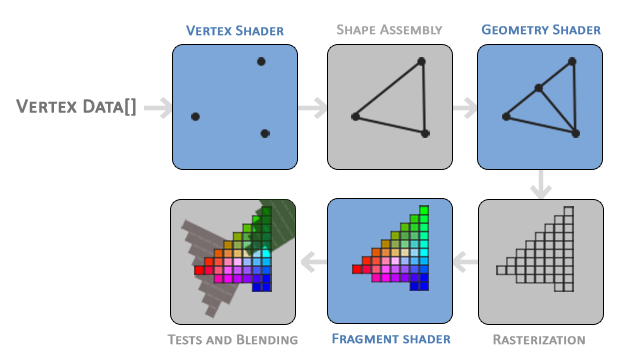
\includegraphics[width=12cm]{pipeline.png}
    }
    \caption{\lr{Graphic pipeline: from learnopengl.com}}
    \label{fig:my_label}
\end{figure}
\vspace*{0.6cm}

    به طور کلی وظیفه \lrit{Vertex Shader} انتقال یک نقطه از فضای \lr{NDC} به فضای دیگر است، غالبا این فضا همان جهان بازی یا برنامه سه بعدی است، برای \lr{Transform} کردن فضای بازیبه فضایی دیگر از ماتریس ها استفاده می شود، به طوری که هر فضا دارای یک \lr{Transformation Matrix}  است، برای رسم کردن مثلث ما نیازی به تغییر فضا نداریم و در \lr{NDC} ادامه می دهیم.
    یک \lr{Vertex shader} ساده به صورت زیر است:

    \begin{LTR}
    \small
        \begin{lstlisting}[style=C++Style,caption=\lrit{basic vertex shader}]
#version 330 core
layout (location = 0) in vec3 aPos;

void main()
{
    gl_Position = vec4(aPos.x, aPos.y, aPos.z, 1.0);
}
        \end{lstlisting}
    \end{LTR}
    \normalsize
    \vspace*{0.3cm}

    کد بالا ساده ترین مدل برای استفاده از \lr{vertex shader} است، این کد به زبان \lr{GLSL(OpenGL Shading Language)} نوشته شده است، در خط اول ما نوع ویژگی ها را که پیش تر توضیح داده بودیم
    را مشخص کرده ایم، خط 2 یک متغیر از نوع \lr{vec3} به اسم \lr{aPos} تعریف کرده ایم، با استفاده از \lrit{layout (location = 0)} در این خط مشخص کرده ایم که این متغیر در حافظه در چه موقعیتی قرار میگیرد، این ویژگی برای وقتی که بخواهیم مقادیر دیگری به جز مختصات نقطه، در یک آرایه ذخیره کنیم و به کارت گرافیک دهیم کارایی دارد.
    در نهایت متغیر \lr{(gl\_Position)} که نشان دهنده مکان این نقطه که در حال پردازش است می باشد را به وسیله مقادیری که از کد  \lr{C} خواندیم و مقدار 1 مقداردهی کردیم، مقدار چهارم در این فضا کاربردی ندارد اما در فضای سه بعدی و در \lr{perspective view} به کار ما می آید.\par
    مرحله بعد ساختن یک \lr{Fragment shader} است، وظیفه این بخش از \lr{pipeline} انجام محاسبات و تعیین رنگ پیکسل می باشد، تمامی محاسبات مربوط به نور، سایه، بازتاب و افکت های گرافیکی غالبا در این مرحله انجام می شود، البته این مقادیر در مراحل بعد ممکن است تغییر کنند.
    یک \lr{fragment shader} ساده به صورت زیر است:

    \newpage
    \begin{LTR}
    \small
        \begin{lstlisting}[style=C++Style,caption=\lrit{basic fragment shader}]
#version 330 core
out vec4 FragColor;

void main()
{
    FragColor = vec4(1.0f, 0.5f, 0.2f, 1.0f);
}
        \end{lstlisting}
    \end{LTR}
    \normalsize
    \vspace*{0.3cm}
    کد بالا مقدار خروجی برای رنگ این \lr{fragment} را برابر با مقداری ثابت قرار می دهد، نوع متغیر \lr{FragColor} از نوع \lr{vec4} تعریف شده و مقادیری که دریافت کرده به ترتیب معنی \lr{red, green, blue, alpha} را می دهند، مقادیر باید بین صفر و یک باشند.\par
    حالا هر کدام از کد های بالارا \lr{compile} می کنیم و سپس به برنامه اصلی که روی \lr{Gpu} قرار می گیرد متصل می کنیم، این برنامه را \lr{shader program} می نامیم، قطعه کد پایین مراحل \lr{compile} و \lr{link} کردن \lr{shader program} را نشان می دهد.

    \begin{LTR}
    \small
        \begin{lstlisting}[style=C++Style,caption=\lrit{compile and link shaders to shader program}]
// hold Vertex shader ID
unsigned int vertexShader;
// create a shader of vertex type
vertexShader = glCreateShader(GL_VERTEX_SHADER);
// upload source code
glShaderSource(vertexShader, 1, &vertexShaderSource, NULL);
// compile vertex shader source
glCompileShader(vertexShader);
// -------------------------------------------------
// hold Fragment shader ID
unsigned int fragmentShader;
//create a shader of frament type
fragmentShader = glCreateShader(GL_FRAGMENT_SHADER);
// upload source
glShaderSource(fragmentShader, 1, &fragmentShaderSource, NULL);
// compile fragment shader source
glCompileShader(fragmentShader);
// -------------------------------------------------
// hold shader program ID
unsigned int shaderProgram;
// create a shader program
shaderProgram = glCreateProgram();
// attach vertex shader to program
glAttachShader(shaderProgram, vertexShader);
// attach fragment shader to program
glAttachShader(shaderProgram, fragmentShader);
glLinkProgram(shaderProgram); // link the program
        \end{lstlisting}
    \end{LTR}
    \normalsize
    \vspace*{0.3cm}

    حالا می توانیم از این \lr{shader program} برای تصویر کردن داده ها استفاده کنیم، در بخش بعد داده ها را بر روی \lr{Gpu} بارگزاری می کنیم.

\newpage
\subsection*{\lr{Upload Data to GPU}}
\noindent
\normalsize
    برای استفاده از مشخصات نقاطی که تعریف کردیم باید آن هارا روی \lr{memory} کارت گرافیک آپلود کنیم، انتقال اطلاعات بین \lr{cpu} و \lr{gpu} نسبتا کند است، پس سعی می کنیم اطلاعات هر چه بیشتری را در یک بار انتفال منتقل کنیم، برای مدیریت حافظه بر روی کارت گرافیک از \lr{vbo(vertex buffer object)} استفاده می کنیم، این بافر ها قابلیت نگهداری تعداد زیادی از داده ها را داند، برای ساختن یک \lr{buffer} در \lr{opengl} و نگهداری مشخصه بافر ایجاد شده به صورت زیر عمل می کنیم:

    \begin{LTR}
    \small
        \begin{lstlisting}[style=C++Style,caption=\lrit{creating a buffer object}]
unsigned int VBO;
glGenBuffers(1, &VBO);
        \end{lstlisting}
    \end{LTR}
    \normalsize
    \vspace*{0.3cm}

    برای استفاده کردن از این بافر و ارسال اطلاعات باید آن را \lr{bind} کنیم:
    \begin{LTR}
    \small
        \begin{lstlisting}[style=C++Style,caption=\lrit{binding to target gl\_array\_buffer}]
glBindBuffer(GL_ARRAY_BUFFER, VBO);
        \end{lstlisting}
    \end{LTR}
    \normalsize
    \vspace*{0.3cm}

    حالا که بافر \lr{bind} شده است، می توانیم داده هایی که در آرایه \lr{vertices} تعریف کردیم را به \lr{gpu memory} منتقل کنیم:
        \begin{LTR}
    \small
        \begin{lstlisting}[style=C++Style,caption=\lrit{uploading data for static draw}]
glBufferData(GL_ARRAY_BUFFER,
             sizeof(vertices),
             vertices,
             GL_STATIC_DRAW);
        \end{lstlisting}
    \end{LTR}
    \normalsize
    \vspace*{0.3cm}

    حالا داده های ما بر روی \lr{gpu} قرار گرفته اند، آرگومان آخری که به تابع بالا دادیم به این معنی است که این داده ها مستعد تغییر نیستند، یعنی نوشتن بر روی آن ها زیاد صورت نمی گیرد اما باید برای خوانده شدن به سرعت در دسترس باشند زیرا به مراتب خوانده می شوند، این به گرافیک کمک می کند تا داده هارا در جایی از حافظه قرار دهد تا این ویژگی ها را داشته باشد.

    داده هایی که بر روی کارت گرافیک دادیم داده خام هستند، باید برای \lr{vertex shader} مشخص کنیم که به چه صورت باید داده هارا تفسیر کند، برای استفاده از ویژگی \lr{attribute} ها در \lr{vertex shader} باید نوع تفسیر داده هارا نیز به صورت دستی مشخص کنیم، به اینکار \lr{Linking Vertex Attribute} می گویند.

    \vspace*{0.6cm}
\begin{figure}[ht]
    \centering
    \href{https://learnopengl.com}{
        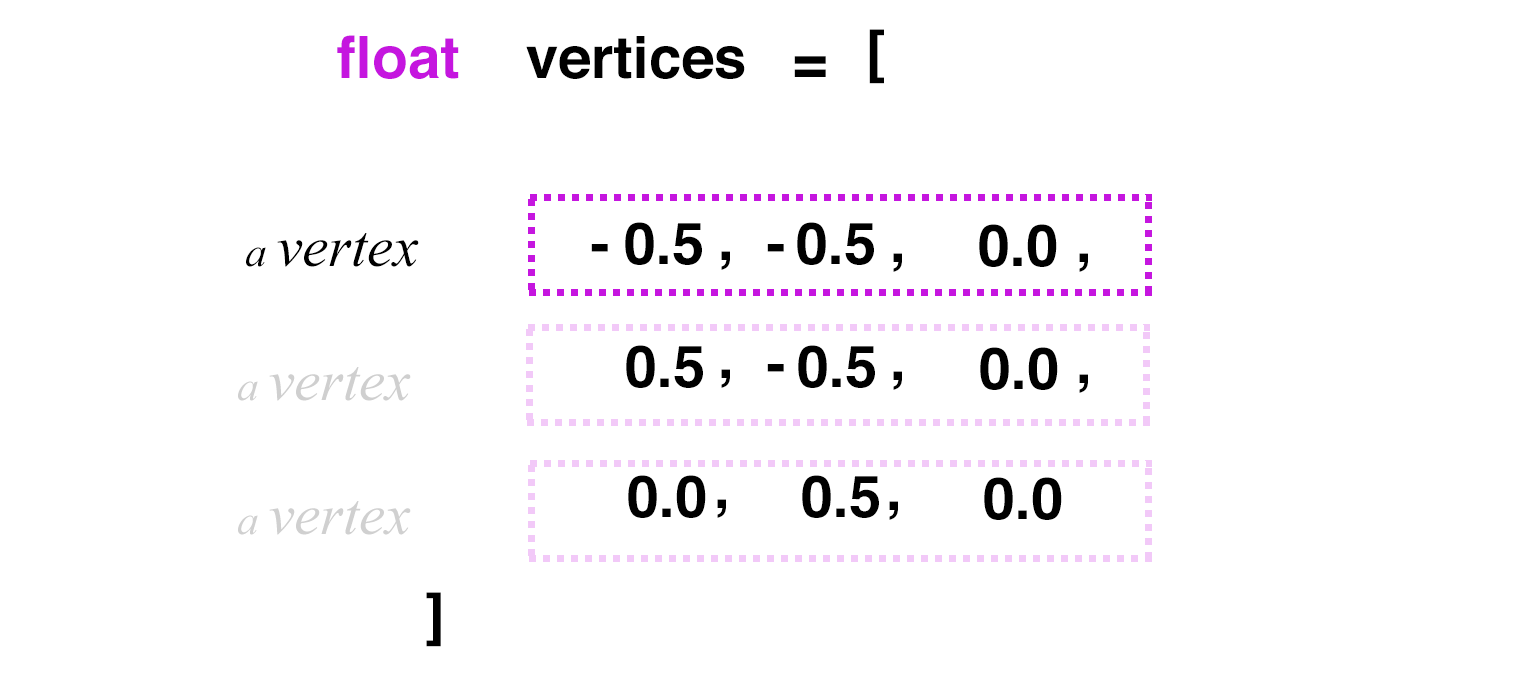
\includegraphics[width=12cm]{images/shm-linking-vertex-attribute.png}
    }
    \caption{\lr{Graphic pipeline: from learnopengl.com}}
    \label{fig:my_label}
\end{figure}
\vspace*{0.6cm}

    برای انجام اینکار باید مقدار چند ویژگی را بدانیم:
\begin{persian}
    \begin{enumerate}
      \item اولین آرگومان برابر با مقداری است که برای متغیر \lr{aPos} در \lr{vertex shader} به وسیله \lr{layout (location = 0)} مشخص کردیم که در این مورد برابر با صفر است.
      \item آرگومان دوم مشخص کننده تعداد متغیر های است که باید به عنوان یک \lr{vertex} شناسایی شوند، این مقدار برای مثال ما برابر 3 است.
      \item این آرگومان مشخص کننده نوع داده هایی است که بارگزاری شده، در این مورد \lr{float} است.
      \item مشخص می کند که داده ها نیاز به نرمال سازی دارند یا خیر.
      \item این مقدار مشخص می کند چند \lr{byte} داده باید برای این \lr{vertex} خوانده شود، به این مقدار \lr{stride} می گویند.
      \item مقدار آخر در مورد مثال ما کاربرد ندارد، در مثال های بعدی می بینیم که مقادیر مربوط به رنگ و دیگر ویژگی های یک نقطه را در به صورت پیوسته در آرایه \lr{vertices} اضافه می کنیم، آنگاه باید از \lr{offset} برای مشخص کردن هر کدام از این ویژگی ها استفاده کنیم.
    \end{enumerate}
\end{persian}

    شکل 3.1 متناسب با توضیحات ساخته شده.

    \begin{LTR}
    \small
        \begin{lstlisting}[style=C++Style,caption=\lrit{link vertex attribute to vertex data}]
glVertexAttribPointer(
    0, // layout (location = 0)
    3, // 3 value for this vertex exists
    GL_FLOAT, // type of each value in vertex
    GL_FALSE, // no need to normalize data
    3 * sizeof(float), // 3 (size of) float in each vertex
    (void*)0  //no offset
    );

glEnableVertexAttribArray(0);
        \end{lstlisting}
    \end{LTR}
    \normalsize
    \vspace*{0.3cm}

    در پروژه های بزرگ تر انجام دادن این عملیات برای تک تک اشیاء موجود در بازی بیهوده و زمان گیر است، برای همین از یکی دیگر از انواع بافر ها به اسم \lr{vertex array object} استفاده می کنیم، این بافر تمامی مراحل قبل و فعال سازی \lr{vertex attribute} ها را ذخیره می کند و دفعات بعد نیازی به انجام تمامی این مراحل نیست و ما فقط باید \lr{VAO} را \lr{bind} کنیم:

    \begin{LTR}
    \small
        \begin{lstlisting}[style=C++Style,caption=\lrit{link vertex attribute to vertex data}]
unsigned int VAO;
glGenVertexArrays(1, &VAO);
// 2. copy our vertices array in a buffer for OpenGL to use
glBindBuffer(GL_ARRAY_BUFFER, VBO);
glBufferData(GL_ARRAY_BUFFER, sizeof(vertices), vertices, GL_STATIC_DRAW);
// 3. then set our vertex attributes pointers
glVertexAttribPointer(0, 3, GL_FLOAT, GL_FALSE, 3 * sizeof(float), (void*)0);
glEnableVertexAttribArray(0);

        \end{lstlisting}
    \end{LTR}
    \normalsize
    \vspace*{0.3cm}


    حالا می توانیم با استفاده \lr{shader program} که \lr{vao} مثلث را بر روی صفحه رسم کنیم، این کار را در بخش بعدی انجام می دهیم.

\newpage
\subsection*{\lr{Render Loop}}
\noindent
\normalsize
    حالا برای رسم کردن مثلث نیاز به کدهای زیر داریم:

    \begin{LTR}
    \small
        \begin{lstlisting}[style=C++Style,caption=\lrit{link vertex attribute to vertex data}]
glUseProgram(shaderProgram);
glBindVertexArray(VAO);
glDrawArrays(GL_TRIANGLES, 0, 3);
        \end{lstlisting}
    \end{LTR}
    \normalsize
    \vspace*{0.3cm}

    ابتدا \lr{shader program} را فعال می کنیم، سپس \lr{VAO} که ساختیم را \lr{bind} می کنیم، حالا تمامی داده ها و تفسیر ها آماده هستند، برای رسم از تابع خط آخر می خواهیم که با داده ها تشکیل مثلث بدهد، ابتدای و انتهای بایت هایی که باید از \lr{vertex array} بخواند را مشخص می کنیم، پس کامپایل کردن و اجرای برنامه با شکل زیر رو به رو می شویم.

\vspace*{0.3cm}
\begin{figure}[ht]
    \centering
    \href{https://learnopengl.com}{
        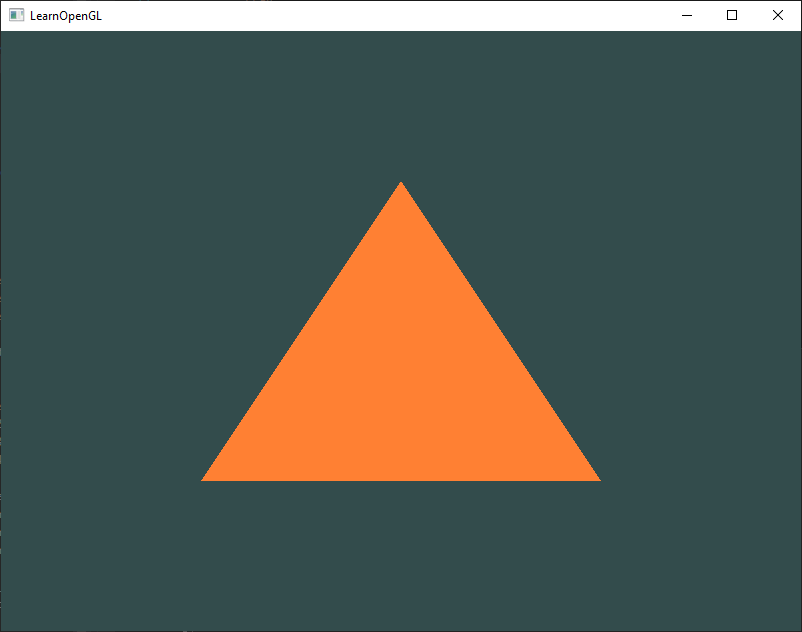
\includegraphics[width=10cm]{images/hellotriangle.png}
    }
    \caption{\lr{hello triangle}}
    \label{fig:my_label}
\end{figure}
\vspace*{0.3cm}

\newpage
    برای اینکه بتوانیم دیگر ویژگی های مدل هارا به \lr{Gpu} ارسال کنیم و از آن ها استفاده کنیم می توانیم از چند \lr{attribute} یا از نوعی از متغیر ها به اسم \lr{uniform} استفاده کنیم، در ابتدا برای افزودن رنگ به هر کدام از \lr{vertex} ها از \lr{attribute} های \lr{vertex shader} استفاده می کنیم، برای این کار کد \lr{vertex shader}  را به شکل زیر تغییر می دهیم:

    \begin{LTR}
    \small
        \begin{lstlisting}[style=C++Style,caption=\lrit{declare and use aColor}]
#version 330 core
layout (location = 0) in vec3 aPos;
layout (location = 1) in vec3 aColor

out vec3 ourColor;

void main()
{
    gl_Position = vec4(aPos, 1.0);
    ourColor = aColor
}
        \end{lstlisting}
    \end{LTR}
    \normalsize
    \vspace*{0.3cm}

    و کد \lr{fragment shader} را به شکل زیر می نویسیم تا بتوانیم از مقادیر رنگ استفاده کنیم:
    \begin{LTR}
    \small
        \begin{lstlisting}[style=C++Style,caption=\lrit{render fragment with color from vertex shader}]
#version 330 core
out vec4 FragColor;
in vec3 ourColor;

void main()
{
    FragColor = vec4(ourColor, 1.0);
}
        \end{lstlisting}
    \end{LTR}
    \normalsize
    \vspace*{0.3cm}

    حالا داده های مربوط به رنگ هر \lr{vertex} را در انتهای داده های مربوط به همان \lr{vertex} اضافه می کنیم، کد به شکل زیر تغییر می کند:
    \begin{LTR}
    \small
        \begin{lstlisting}[style=C++Style,caption=\lrit{position and color data in one array}]
float vertices[] = {
    // positions         // colors
     0.5f, -0.5f, 0.0f,  1.0f, 0.0f, 0.0f,   // bottom right
    -0.5f, -0.5f, 0.0f,  0.0f, 1.0f, 0.0f,   // bottom left
     0.0f,  0.5f, 0.0f,  0.0f, 0.0f, 1.0f    // top
};
        \end{lstlisting}
    \end{LTR}
    \normalsize
    \vspace*{0.3cm}

    داده هارا به شکل قبل به \lr{VBO} اضافه می کنیم، سپس \lr{VAO} را \lr{bind} می کنیم، یک مرحله جدید در \lr{link vertex attribute} برای رنگ ها اضافه شده است، این مرحله به شکل زیر است:
       \begin{LTR}
    \small
        \begin{lstlisting}[style=C++Style,caption=\lrit{position and color data in one array}]
// position attribute
glVertexAttribPointer(0, 3, GL_FLOAT, GL_FALSE, 6 * sizeof(float), (void*)0);
glEnableVertexAttribArray(0);
// color attribute
glVertexAttribPointer(1, 3, GL_FLOAT, GL_FALSE, 6 * sizeof(float), (void*)(3* sizeof(float)));
glEnableVertexAttribArray(1);
        \end{lstlisting}
    \end{LTR}
    \normalsize
    \vspace*{0.3cm}

    همانطور که می بینیم در این مرحله متغیر های مربوط \lr{stride} و \lr{offset} به شکل جدید برای استفاده از و تفسیر تمام داده برای \lr{gpu} تغییر کرده اند، در خط 5 کد بالا متغیر \lr{offset} نشان دهنده این است که برای خواندن سه مقدار برای رنگ، باید \lr{offset} را برابر 3 قرار دهیم تا سه مقدار اول که برای داده های مکان نقطه تعریف کرده ایم در نظر نگیرد، همچنین متغیر \lr{stride} را برابر با شش قرار دادیم، این به معنی این است که هر 6 مقدار در آرایه بیانگر ویژگی ها برای یک نقطه متفاوت است.\par
    رنگ مثلث به صورت زیر تغییر می کند:

\vspace*{0.3cm}
\begin{figure}[ht]
    \centering
    \href{https://github.com/devprofile98/shm}{
        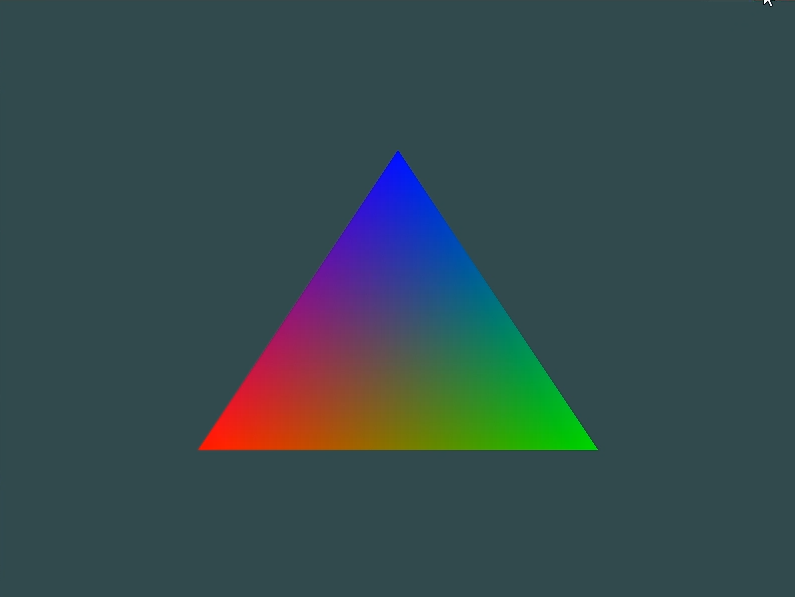
\includegraphics[width=10cm]{images/colorfultriangle.png}
    }
    \caption{\lr{colorful triangle}}
    \label{fig:my_label}
\end{figure}
\vspace*{0.3cm}
    در مثال بالا \lr{opengl} مقدار رنگ سه نقطه را از ما دریافت کرد و به صورت خودکار مقدار رنگ بین این نقاط را به صورت خطی \lr{interpolate} کرد.\par
    این روش برای مدل ها و اشیاء سه بعدی نه تنها کاربردی نیست بلکه هزینه زیادی دارد، روش بهتر برای مقدار دهی به رنگ و ایجاد جزئیات برای اشیاء استفاده از \lr{texture} ها است، در بخش بعد درباره تکسچرها توضیح می دهم.

\newpage
\subsection*{\lr{Textures}}
\noindent
\normalsize
    تصور کنید می خواهیم یک دیوار را شبیه سازی کنیم، دیوار را می توانیم با چهار نقطه با استفاده از \lr{EBO( element buffer object)} بسازیم، این چهار نقطه برای ما تشکیل یک مربع یا مستطیل(دو مثلث که از وتر بر روی یکدیگر قرار گرفته اند) بسته به موقعیت نقاط می دهند. مرحله بعدی اضافه کردن جزئیات رنگ یعنی شکل آجر ها بر روی دیوار است، این کار به سادگی امکان پذیر نیست، زیرا ما فقط قابلیت تعیین چهار رنگ برای چهار نقطه را داریم، پس نمی توانیم با چهار رنگ و \lr{linear interpolation} که \lr{opengl} بین این رنگ ها انجام می دهد یک دیوار آجری رندر کنیم، راه حل این مشکل استفاده از یک \lr{texture} است، به صورت ساده می توانیم عکس یک دیوار آجری را به \lr{opengl} بدهیم و بخواهیم که به ازای هر \lr{fragment} از یکی از \lr{pixel} های عکسی که ما به عنوان \lr{texture} آپلود کرده ایم استفاده کند. برای استفاده از یک \lr{texture} ما باید مراحل زیر را انجام دهیم.

\begin{persian}
    \begin{enumerate}
      \item اضافه کردن \lr{texture coordinates} به آرایه داده ها و آپلود آن بر روی \lr{vertex attribute}.
      \item خواندن عکس از حافظه و آپلود کردن آن بر روی \lr{Gpu}.
      \item تنظیم کردن حداقل برخی از ویژگی های تکسچر که به صورت پیشفرض مقداری ندارند.
      \item استفاده از توابع \lr{GLSL} برای \lr{sample} کردن \lr{texture}
    \end{enumerate}
\end{persian}

\newpage

    در مرحله اول مقادیر \lr{texture coordinate} را به آرایه داده ها اضافه می کنیم:
    \begin{LTR}
    \small
        \begin{lstlisting}[style=C++Style,caption=\lrit{position and color data in one array}]
float vertices[] = {
    // positions          // colors           // texture coords
     0.5f,  0.5f, 0.0f,   1.0f, 0.0f, 0.0f,   1.0f, 1.0f,
     0.5f, -0.5f, 0.0f,   0.0f, 1.0f, 0.0f,   1.0f, 0.0f,
    -0.5f, -0.5f, 0.0f,   0.0f, 0.0f, 1.0f,   0.0f, 0.0f,
    -0.5f,  0.5f, 0.0f,   1.0f, 1.0f, 0.0f,   0.0f, 1.0f
};
        \end{lstlisting}
    \end{LTR}
    \normalsize
    \vspace*{0.3cm}

    دقت کنید که باید مراحل \lr{linking vertex attribute} را برای مقادیر جدید انجام دهیم.

    حالا عکس را از دیسک می خوانیم، برای این کار از \href{https://github.com/nothings/stb}{\lrbold{stbi\_image}} استفاده می کنیم، این کتابخانه به صورت \lr{single header library} در دسترس است، این گونه کتابخانه در یک فایل نوشته شده اند و استفاده درست از آن ها با استفاده از \lr{define} است.

    پس از بازکردن عکس در کد باید یک \lr{texture} بسازیم، ابتدا یک شی\lr{texture} می سازیم و سپس می توانیم داده های عکسی که خواندیم را بر روی تکسچری که ساختیم \lr{upload} کنیم، اینکار به شیوه زیر انجام می گیرد:

    \begin{LTR}
    \small
        \begin{lstlisting}[style=C++Style,caption=\lrit{load and upload data to gpu}]
unsigned int texture; // hold texture ID
glGenTextures(1, &texture); // create texture object on gpu
// bind texture to 2d_texture target
glBindTexture(GL_TEXTURE_2D, texture);
// upload image data to texture that is bound i.e texture variable
glTexImage2D(GL_TEXTURE_2D, 0, GL_RGB, width, height,
    0, GL_RGB, GL_UNSIGNED_BYTE, data); // data is the Image
// generating mip maps for this texture
glGenerateMipmap(GL_TEXTURE_2D);
        \end{lstlisting}
    \end{LTR}
    \normalsize
    \vspace*{0.3cm}


    نیاز داریم که برخی مقادیر را برای \lr{texture} تنظیم کنیم وگرنه با یک تکسچر سیاه رو به رو می شویم، مقادیر زیر برای تنظیم تکرار شدن تصویر در جهات مختلف و مشخص کردن الگوریتم مناسب برای زمان کوچک نمایی با بزرگ نمایی تصویر است، به صورت زیر این مقادیر را تنظیم می کنیم:

    \begin{LTR}
    \small
        \begin{lstlisting}[style=C++Style,caption=\lrit{set minimum setting for a texture}]
glTexParameteri(GL_TEXTURE_2D, GL_TEXTURE_WRAP_S, GL_REPEAT);	
glTexParameteri(GL_TEXTURE_2D, GL_TEXTURE_WRAP_T, GL_REPEAT);
glTexParameteri(GL_TEXTURE_2D, GL_TEXTURE_MIN_FILTER, GL_LINEAR_MIPMAP_LINEAR);
glTexParameteri(GL_TEXTURE_2D, GL_TEXTURE_MAG_FILTER, GL_LINEAR);
        \end{lstlisting}
    \end{LTR}
    \normalsize
    \vspace*{0.3cm}

    مختصات تکسچر را در \lr{vertex shader} به صورت یک \lr{vertex attribute} جدید تعریف می کنیم و به مرحله \lr{fragment shader} می فرستیم، ارسال این داده ها بین مراحل مختلف \lr{pipeline} را با استفاده از متغیر هایی که با \lr{in, out} تعریف می شوند انجام می دهیم، به این صورت که متغیر را در مرحله ای که زودتر انجام می شود(در این مورد \lr{vertex shader}) به صورت \lr{out} تعریف می کنیم و در مرحله بعد آن را با \lr{in} تعریف می کنیم، دقت کنید باید نام متغیر دقیقا برابر باشد، کد زیر به \lr{vertex shader} اضافه می کنیم:

       \begin{LTR}
    \small
        \begin{lstlisting}[style=C++Style,caption=\lrit{vertex shader to use texture}]
layout (location = 2) in vec2 aTexCoord;
out vec2 TexCoord; // vec2 because of 2d image
...
void main()
{
    ....
    TexCoord = aTexCoord;
}
        \end{lstlisting}
    \end{LTR}
    \normalsize
    \vspace*{0.3cm}

    در قمست \lr{fragment shader} نیز کد به شکل زیر تغییر می کند:

    \begin{LTR}
    \small
        \begin{lstlisting}[style=C++Style,caption=\lrit{fragment shader to use texture}]
#version 330 core
out vec4 FragColor;
...
in vec2 TexCoord;

uniform sampler2D ourTexture;

void main()
{
    //built in texture function for sampling texture to fragment
    FragColor = texture(ourTexture, TexCoord);
}
        \end{lstlisting}
    \end{LTR}
    \normalsize
    \vspace*{0.3cm}

    نتیجه به شکل زیر در می آید:

\vspace*{0.3cm}
\begin{figure}[ht]
    \centering
    \href{https://github.com/devprofile98/shm}{
        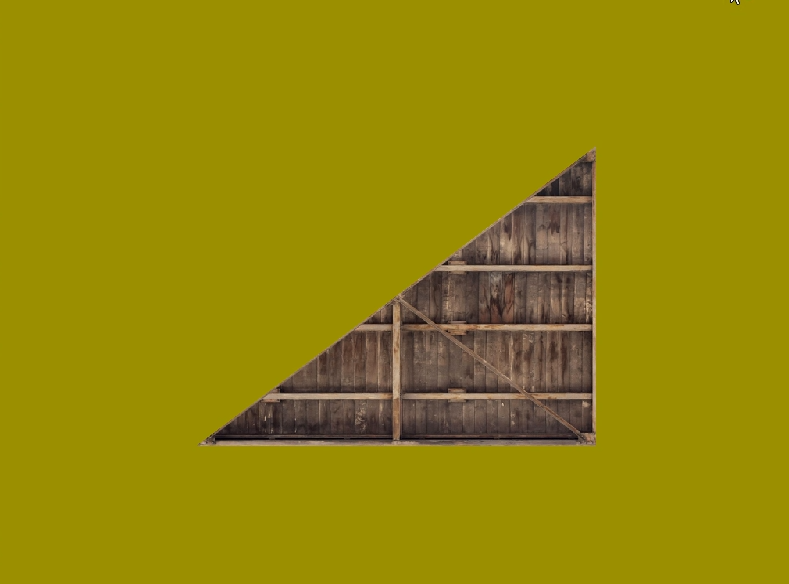
\includegraphics[width=13cm]{images/texturedtriangle.png}
    }
    \caption{\lr{colorful triangle}}
    \label{fig:my_label}
\end{figure}
\newpage


% end of section -------------------

% section start --------------------
\vspace*{6.0cm}
\addcontentsline{toc}{section}{دوربین و حرکت در جهان}
\section*{\huge{دوربین و حرکت در جهان}}
\vspace*{0.6cm}
\subsection*{\lr{Transformations}}
\noindent
\normalsize

    می توانیم با دو مثلث یک مربع درست کنیم، و با شش مربع یک مکعب تشکیل دهیم، و با استفاده از یک حلقه و چند \lr{draw call} چند مکعب بسازیم، اما در حال حاظر این کار فایده ای ندارد چون تمامی مکعب ها بر روی یکدیگر قرار می گیرند و. ما فقط یک مکعب را به صورت دو بعدی می بینیم، برای دیدن یک مکعب به یک محیط که شبیه ساز سه بعد باشد نیاز داریم، می توانیم مختصات مکعب هارا در حلقه تغییر دهیم و در قسمت های مختلف صفحه رندر کنیم، به این کار \lr{translate} کردن می گوییم، این عمل را با استفاده از یک ماتریس
    $4x4$ 
    انجام می دهیم، یک \lr{translation matrix} به شکل زیر است:\par
\begin{center}
\setlength\arraycolsep{5pt}
\renewcommand{\arraystretch}{0.75}
	$$
	\begin{bmatrix}
	1 & 0 & 0 & x \\
	0 & 1 & 0 & y \\
	0 & 0 & 1 & z \\
    0 & 0 & 0 & 1
	\end{bmatrix}
	\quad
	$$
\end{center}
    
    مقادیر $(x, y, z)$ به ترتیب نشان دهنده تغییرات بر بردار متناسب با خود هستند، می توانیم هر کدام از نقاط مدل خود را توسط ماتریس بالا به نقطه جدید خود منتقل کنیم، ماتریس های \lr{rotation} و \lr{scale} نیز به ترتیب برای چرخش حول محور های مشخص و تغییر مقیاس استفاده می شوند، به حاصل ضرب این سه جزء یک \lr{model matrix} می گویند.\par
    پس از ضرب کردن \lr{model} در مختصات هر نقطه از شکل خود، اصطلاحا مختصات نقاط را در \lr{local space} به \lr{world space} برده ایم.\par
    برای انجام عملیات ریاضی مربوط به \lr{opengl} بر روی \lr{cpu} از کتابخانه \lrbold{GLM} استفاده می کنیم، این کتابخانه دارای کلاس ها و توابعی است که نمایانگر ساختار های ریاضیاتی مانند \lr{vector} ها و \lr{matrix} ها است، همچنین تعداد دیگری از توابع را داراست که برای ساده سازی کار ما فراهم شده اند، یکی از این توابع \lr{glm::LookAt} است، می  توانیم از این کلاس برای تشکیل یک \lr{view matrix} استفاده کنیم که نشانگر \lrbold{Camera} است.\par
    \vspace*{0.6cm}
    \subsubsection*{\lr{Camera}}
    \vspace*{0.3cm}
    
    در دنیای واقعی اگر جسمی از ما فاصله بیشتری داشته باشد کوچکتر دیده می شود، این تعریف بسیار ساده و مختصری از \lr{perspective view} است، نور یازتاب شده از اجسام به مرکز چشم ما برمیگردد و اجسامی که نزدیک تر هستند بزرگتر دیده می شوند، در مقابل این مدل \lr{orthographic views} قرار دارند، در این مدل که در طراحی های صنعتی بیشتر کاربر دارد و در دنیای واقعی وجود ندارد، هر کدام از \lr{pixel} های صفحه پرتویی به صورت جداگانه از خود ساطع می کنند، همه این پرتوها موازی هستند و در نتیجه فاصله جسم از بیننده در نحوه دیدن شکل تاثیری ایجاد نمی کند، ما برای داشتن یک فضای سه بعدی واقع گرایانه از \lr{perspective projection} استفاده می کنیم، برای ساختن این ماتریس از \lr{GLM} به شکل زیر استفاده می کنیم:
    
    \begin{LTR}
    \small
        \begin{lstlisting}[style=C++Style,caption=\lrit{fragment shader to use texture}]
glm::mat4 proj = glm::perspective(glm::radians(45.0f), (float)width/(float)height, 0.1f, 100.0f);
        \end{lstlisting}
    \end{LTR}
    \normalsize
    \vspace*{0.3cm}
    
    آرگومان اول مقددار \lr{fov (field of view)} است، این مقدار به نحوی مقدار بزرگنمایی تصویر ما را مشخص می کند، آرگومان دوم \lr{aspect ratio} دوربین و مقادیر سوم و چهارم به ترتیب فاصبه صفحه نزدیک و دور را مشخص می کنند، این مشخصات تشکیل یه فضای سه بعدی می دهند که هر چه خارج از آن باشد قابل مشاهده نیست، همچنین دید \lr{perspective} را به ما ارائه می کنند.
    شکل زیر بیانگر این موضوع است:
    
\begin{figure}[ht]
    \centering
    \href{https://learnopengl.com}{
        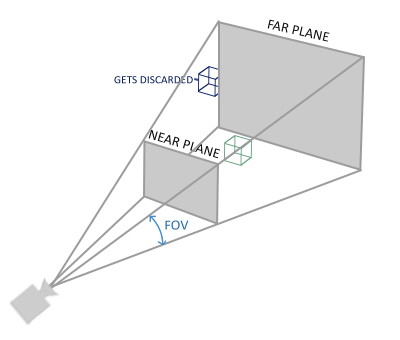
\includegraphics[width=10cm]{images/perspective_frustum.png}
    }
    \caption{\lr{perspective frustum}}
    \label{fig:my_label}
\end{figure}
    
\part{فیزیک}
\begin{center}
    \chapter{\lr{Physics}}
\end{center}
\section{\lr{Particles}}
\section{\lr{Rigid Bodies}}

\end{document} 